\renewcommand{\labelenumi}{(\alph{enumi})}

\title{Introduction to Computational Earth Sciences Homework \#4 \\
 Stanford GP $257$, Spring $2008$-$09$ }
\lefthead{}
\righthead{}
\footer{}

\author{Instructor: Robert Clapp}

\section{Due Date: 5 pm Friday, 29 May 2009}

\title{MPI Parallel Computing [20 points]}
The purpose of this homework is to use the Message Passing interface (MPI) for parallel computing. Students taking the class for 2 units are required to submit only the first problem. Students enrolled in 3 or 4 units must submit both problems.
\author{Joe Schmoe}
\section{Ping-Pong [10 points]}
In this section of the assignment you will be analyzing the latency and bandwidth of MPI communication. 
Begin the assignment by logging onto \texttt{cees-tool.stanford.edu} and updating
your working subversion directory.

In the \texttt{src} directory you will find a Makefile and shell script \texttt{pingpong.sh} to submit parallel MPI jobs through the CEES grid engine. Log into \texttt{cees-opteron.stanford.edu}, the Linux distributed memory cluster. In the \texttt{src} directory you will find the Ping-Pong example shown in class for both C (\texttt{pingpong.c}) and Fortran 90 (\texttt{pingpong.f90}). To compile the program type 
\begin{quote}
\begin{verbatim}
% make target=pingpong language=c
\end{verbatim}
\end{quote}
or
\begin{quote}
\begin{verbatim}
% make target=pingpong language=f90
\end{verbatim}
\end{quote}
for C and Fortran respectively. To submit the MPI program to the CEES grid engine type
\begin{quote}
\begin{verbatim}
% qsub pingpong.sh
\end{verbatim}
\end{quote}

Generate a plot for each of the following cases illustrating the bandwidth as a function of message size (Figure~\ref{fig:q1}):
\begin{enumerate}
	\item Extend the Ping-Pong program to send messages of size $2^n$ where \mbox{$n = 0,1, \ldots, 20$}. To ensure accuracy of timings, loop over 1000 iterations for each $n$ and print the average time per message size and hop. How do bandwidth and latency depend on the message lengths?
	
	\item Recompute the measurements from (a) with replacing the individual \texttt{MPI\_Send()} and \texttt{MPI\_Recv()} calls with a single \texttt{MPI\_Sendrecv()} call. What changes?
\end{enumerate}

\begin{figure}[h] \centering
  \subfigure[]{
    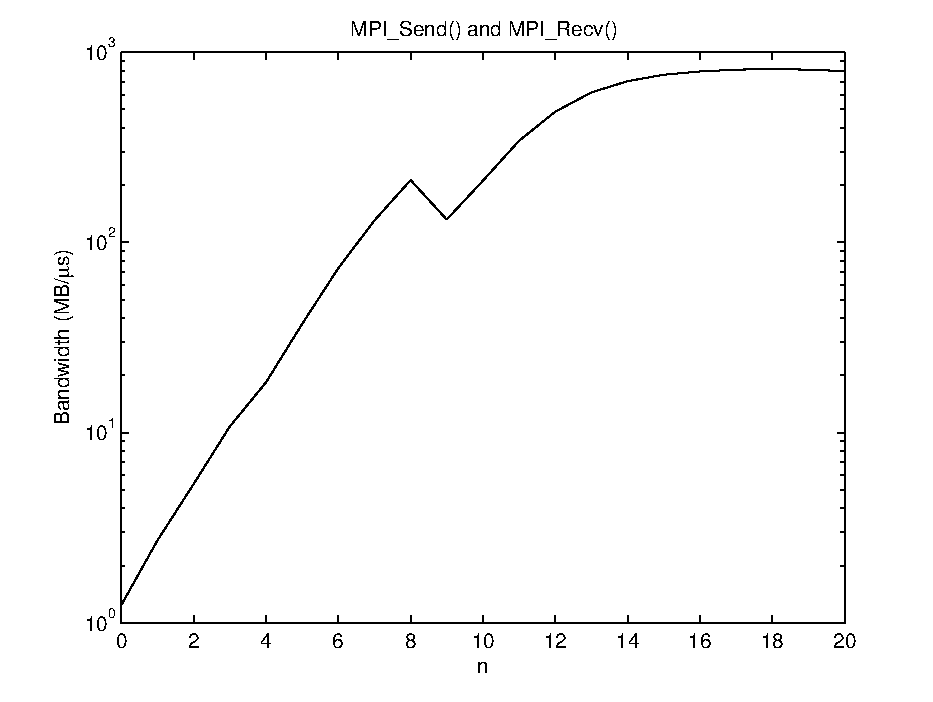
\includegraphics[width=0.47\textwidth]{./Fig/pingpong_block}
  }
  \subfigure[]{
    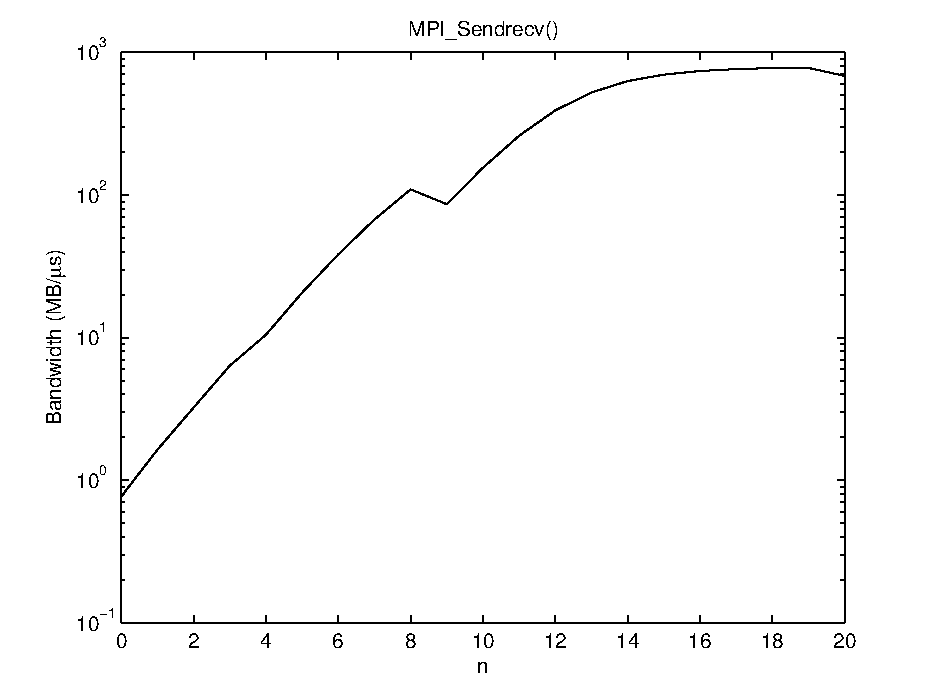
\includegraphics[width=0.47\textwidth]{./Fig/pingpong_sendrecv}
  }
  \caption{.}
  \label{fig:q1}
\end{figure}

\section{Scalar Advection Equation [10 Points]}
Consider the scalar advection equation
\[
  \frac{\partial u}{\partial t} + a \frac{\partial u}{\partial x} = 0 \qquad 0 \le x \le 1
\]
with boundary conditions $u(0, t) = 0$ and initial profile and $u(x,0)= 1 - (10x - 1)^2$ where $x <= 0.2$ and 0 for other values of x.
The equation describes the propagation of a scalar $u$. Assume that the fluid is moving with a constant velocity $a = 0.08$ in the $x$ direction. The exact solution is given by
$ u(x, t) =  1 - [10(x - at) - 1]^2$ for $ 0 \le (x - at)$ and $0$ at other values of $x$.
Discretizing using forward-time (explict Euler) and backward-space for $a > 0$ gives
\[
  \frac{u_j^{n + 1} - u_J^{n}}{\Delta t} + a \frac{u_j^n - u_{j - 1}^n}{\Delta x} + \mathcal{O}(\Delta x, \Delta t) = 0
\]
Therefore
\begin{eqnarray}
  u_j^{n + 1} &= u_j^n - \frac{a \Delta t}{\Delta x}\left(u_{j}^n - u_{j - 1}^{n}\right)+ \mathcal{O}(\Delta x, \Delta t) \\
  &=  u_j^n - \gamma \left(u_{j}^n - u_{j - 1}^{n}\right) \\
  \label{eqn:discretization}
\end{eqnarray}
where $u_0^{n + 1} = 0$. In the above equation $\Delta x = 1/N$ where $N$ is the number of grid cells and
\[
  \gamma = \frac{u\Delta t}{\Delta x}
\]  
For stability the CFL condition requires that $\gamma \le 1$, which implies that the time step $\Delta t$ is bounded by
\[
  \Delta t \le \frac{\Delta x}{a}
\]
Note that for the scalar advection equation, the numerical solution is exact for $\gamma = 1$. The numerical and exact solution for $t = 0$ and $8$ seconds are shown in Figure~\ref{fig:q2_solution}.

\begin{figure}[h] \centering
  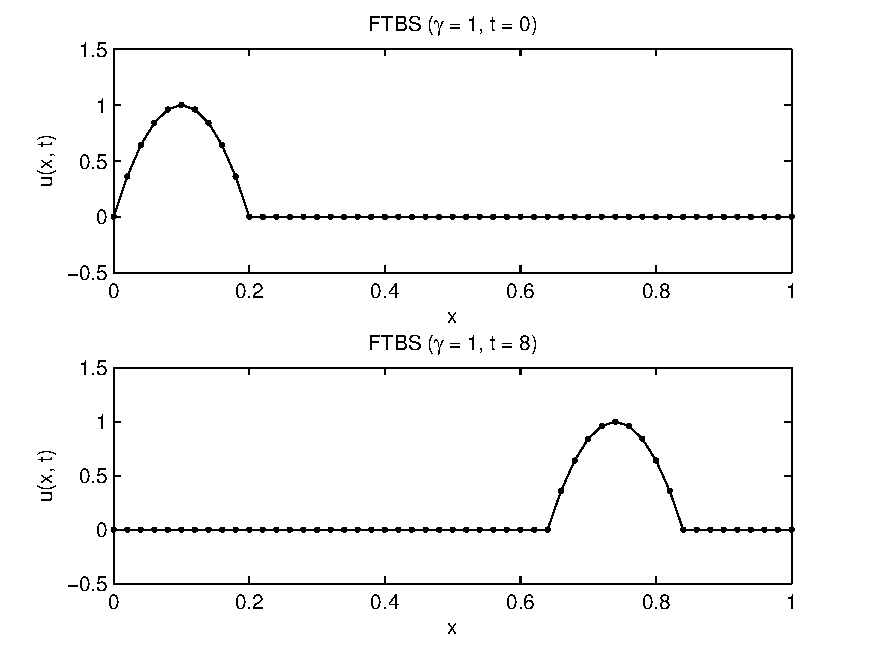
\includegraphics[width=0.60\textwidth]{./Fig/solution}
  \caption{One-dimensional advection equation for forward-time backward-space (FTBS) for $t = 0, \, 8$ with $\Delta x = 0.02$, where \texttt{-} denotes the exact solution and \texttt{o:} the numerical solution. Note that $\|u(x, t) - u^h(x, t)\| = 0$.}
  \label{fig:q2_solution}
\end{figure}

In the \texttt{src} directory you will find serial code for C (\texttt{advection.c}) for solving the one-dimensional advection equation. You are required parallelize the spatial domain using MPI, where you only have to modify the \texttt{main} and \texttt{advection} routines. To compile the C program type
\begin{quote}
\begin{verbatim}
% make target=advection language=c 
\end{verbatim}
\end{quote}
Run the MPI program using $p = 2,\,4,\,8,\,16$ and 32 processors by modifying the submitting the \texttt{advection.sh} script to the CEES grid engine. Reproduce Figure~\ref{fig:q2_performance} for timings are parallel speedup and comment on the results.

\clearpage
\newpage
\subsubsection*{MPI Implementation}
Figure~\ref{fig:q2_decomposition} illustrates the domain decomposition for solving the one-dimensional scalar advection equation on $p$ processors. Referring to equation~\ref{eqn:discretization} the solution of the FTBS discretization is of the form $u^{n + 1}_j = f(u_{j - 1}^n, u_j)$, hence at each time step, processor $i$ has to only communicate with processor $i + 1$, which one requires one ghost cell per sub-domain. The use of \texttt{MPI\_PROC\_NULL} simplifies the code for the boundary regions defined on processor 1 and $p$ for $u(0, t)$ and $u(1, t)$ respectively.

It is strongly advised that you test your MPI implementation using a smaller number of grid cells, ensuring that the output is in agreement with the serial solution. Furthermore for $\gamma = 1$, the error norm is $\|u(x, t) - u^h(x, t)\| = 0$, where $u^h(x, t)$ denotes the numerical solution. Verify your MPI solution initially for one processor, prior to testing on two or more. 
\plot{send}{width=5.0in}{Domain decomposition for the one-dimension advection equation using FTBS discretization which requires only one ghost cell within each subregion corresponding to the value $u_{j - 1}^n$, hence $m = N/p + 2$. At each time-step the $u_{m}^n$ buffer is sent from processor $i$ to the $u_{0}^n$ buffer on processor $i + 1$.}

\subsubsection*{Parallel Performance Analysis}
In an ideal, if computations carried out on $p$ equal parts, the total execution time will be nearly $1/p$ of the time required by a single processor. Let $t_j$ denote the wall clock time required to execute a task with $j$ processors, then the speedup $S_p$, for $p$ processors is defined as
\[
  S_p = \frac{t_1}{t_p}
\]
where $t_1$ is the time required for the most efficient sequential algorithm. Note that this is not the same as running the MPI code using one one processor. Furthermore the computational efficiency using $p$ processors is defined as 
\[
  E_p = \frac{S_p}{p}
\]
where $0 \le E_p \le 1$.

\begin{figure}[h] \centering
  \subfigure[]{
    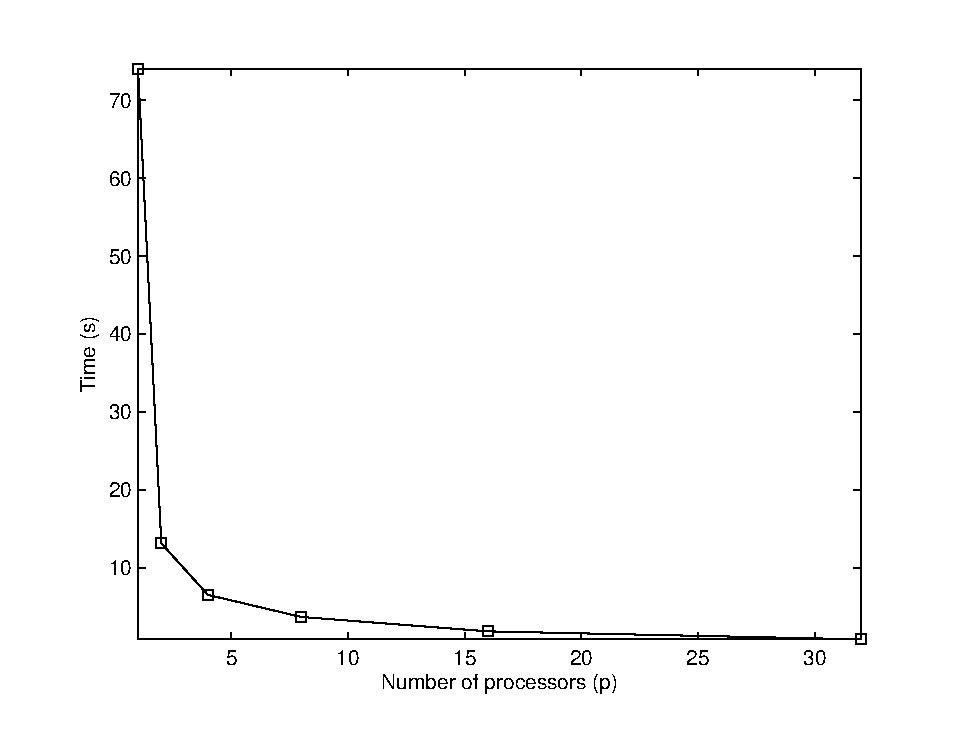
\includegraphics[width=0.47\textwidth]{./Fig/time}
  }
  \subfigure[]{
    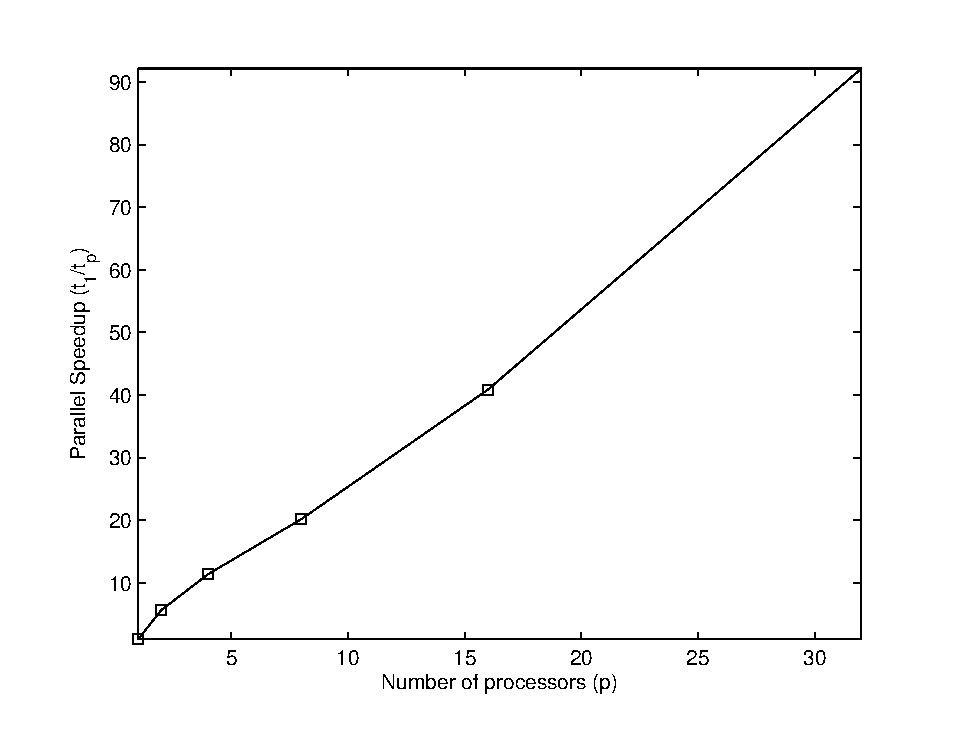
\includegraphics[width=0.47\textwidth]{./Fig/speedup}
  }
  \caption{Parallel performance of the one-dimensional scalar advection equation for (a) timing and (b) speedup.}
  \label{fig:q2_performance}
\end{figure}

